% Springer Nature journal article template, Version 3.1 (December 2024)
% Project: PI-MSCL battery SOH estimation
% Reference style follows the supplied single-column sn-mathphys-num template.

\documentclass[pdflatex,sn-mathphys-num]{sn-jnl}

\usepackage{graphicx}
\usepackage{multirow}
\usepackage{amsmath,amssymb,amsfonts}
\usepackage{booktabs}
\usepackage{siunitx}
\usepackage{array}

% Float rhythm follows the manually polished companion Springer manuscript.
\setcounter{topnumber}{2}
\setcounter{totalnumber}{3}
\renewcommand{\topfraction}{0.95}
\renewcommand{\bottomfraction}{0.95}
\renewcommand{\textfraction}{0.08}
\renewcommand{\floatpagefraction}{0.85}
\setlength{\textfloatsep}{15pt plus 3pt minus 3pt}
\setlength{\floatsep}{13pt plus 3pt minus 3pt}

\raggedbottom

\begin{document}

\title[SOH estimation with sparse cycle-level labels]{Cross-Cell SOH Estimation from Sparse Cycle-Level Labels with a Physics-Informed Multi-Scale CNN-LSTM}

\author[1]{\fnm{Chang} \sur{Liu}}

\author*[1]{\fnm{Congyan} \sur{Chen}}\email{chency@seu.edu.cn}

\affil[1]{\orgdiv{School of Automation}, \orgname{Southeast University}, \orgaddress{\street{No.2 Sipailou}, \city{Nanjing}, \postcode{210096}, \country{China}}}

\abstract{Reference-capacity tests provide reliable state-of-health (SOH) targets, but they are costly to perform at every cycle. Charging features and cycle order can nevertheless remain available between calibrations. Here, we examine whether a soft structural prior can complement reduced numerical supervision in cross-cell SOH estimation. We construct a controlled sparse-label protocol on the fully labelled HUST dataset: cells are separated before model development, then a fixed proportion of cycle-level SOH targets is retained at random within each training cell. Complete feature windows and fully labelled evaluation of unseen test cells are preserved. The proposed physics-informed multi-scale CNN-LSTM (PI-MSCL) combines three temporal convolutional scales, recurrent state modelling, masked data fitting, and a soft monotonicity constraint. A paired $2\times2$ design separates the effects of multi-scale representation and the constraint at retention ratios of 1.0, 0.7, 0.5, and 0.3. Under full supervision, PI-MSCL achieved the lowest mean absolute error (MAE) among eight same-protocol models ($1.556\pm0.044\%$), whereas GRU achieved the lowest root mean squared error and the highest $R^2$. At 30\% retention, attention CNN--LSTM achieved the lowest MAE ($1.567\pm0.087\%$), compared with $1.677\pm0.128\%$ for PI-MSCL. Adding the soft monotonicity constraint reduced PI-MSCL MAE by 0.045 percentage points at 70\% retention and improved the three trajectory-consistency metrics on average. At 30\% retention, it reduced the monotonicity-violation rate by 0.348 percentage points, while paired MAE changes remained mixed. The results identify a conditional accuracy--trajectory-consistency trade-off under a distributed training-label budget, rather than a universal performance advantage.}

\keywords{Lithium-ion battery, state of health, sparse cycle-level supervision, multi-scale CNN-LSTM, soft monotonicity constraint, battery management system}

\maketitle

\section{Introduction}

State of health (SOH) informs safety warnings, lifetime management, and maintenance decisions in lithium-ion battery systems \cite{berecibar2016critical}. Capacity-derived SOH is reliable, but repeated reference-capacity tests are costly. This creates a practical mismatch: operating features are recorded throughout cycling, whereas trustworthy numerical SOH targets are available less frequently. The mismatch is relevant to reuse and second-life assessment, where SOH estimation remains a limiting task \cite{vignesh2024state}.

Data-driven SOH estimators learn health-related patterns from charge and discharge measurements shaped by coupled degradation processes \cite{che2023health,birkl2017degradation}. Sequence models can represent local signal variation and cross-cycle evolution, including LSTM, GRU, convolutional-recurrent, attention, and Transformer-based architectures \cite{hochreiter1997long,liu2023online,zhu2022attention,fan2023online,chen2022state,zhao2023state}. The convolutional component in most of these architectures uses a single kernel size, which fixes one receptive field for every branch of the network. Charging trajectories, however, carry information at several distinct time scales simultaneously: near-adjacent cycles capture transient charge-response variation, intermediate windows capture stage-wise shifts in charge duration and voltage statistics, and longer windows describe the slower drift associated with capacity fade. A fixed-kernel encoder must trade off these scales rather than represent them jointly, which motivates a multi-scale convolutional design as a complementary route to improving feature quality, independent of how densely the resulting representations are supervised. Related work has also used partial charging curves, transfer learning, cycle synchronization, and graph representations to reduce measurement or modelling burdens \cite{lyu2021partial,lu2023deep,ma2022real,zhou2022transfer,zhou2024graph}. Most of these approaches nevertheless rely on dense SOH targets during training.

Recent label-efficient studies address this dependence through few-shot learning, early-life observations, weak labels, semi-supervised transfer, unlabeled charging data, and selective pseudo-labeling \cite{zhang2023fewshot,han2024limited,wang2024weaklabels,qian2026minimal,li2020state,lin2023improving,salucci2023novel,li2026auxiliary}. Their supervision settings are not interchangeable. Labels may be sparse across cells, confined to an early-life prefix, associated with local curve segments, or supplemented by auxiliary signals. A controlled protocol is therefore needed to isolate the contribution of cycle-level SOH targets while holding the available operating features, cell split, and test evaluation fixed.

Trajectory structure offers one route to using the remaining unlabelled cycles. After the early activation region, large upward excursions in an estimated SOH trajectory are inconsistent with the dominant direction of capacity fade, although small recoveries and measurement fluctuations can occur. Physics-informed learning incorporates governing relations or domain constraints into data-driven objectives \cite{raissi2019physics,karniadakis2021physics}. In battery applications, physics-guided models have been used for partial-charge prognostics, stable degradation modelling, and constrained neural estimation \cite{kohtz2022physics,wang2024physics,ye2024method,wen2023physics}. For the present setting, a soft monotonicity constraint is used as a structural prior rather than as an electrochemical degradation model.

Here, we study cross-cell SOH estimation under a controlled sparse cycle-level supervision protocol on the fully labelled HUST dataset. Cells are separated into training, validation, and test subsets before model development. Within each training cell, a fixed proportion of cycle-level targets is retained at random, while feature windows and their temporal order remain available. The protocol therefore tests a distributed training-label budget, not prediction into an unlabelled future segment. We introduce a physics-informed multi-scale CNN-LSTM, termed PI-MSCL, which combines three convolutional receptive fields, recurrent state modelling, masked data fitting, and soft monotonicity regularisation. A paired $2\times2$ experiment separates the effects of multi-scale representation and the structural prior across four retention ratios. We report point-estimation metrics together with trajectory-consistency metrics and same-protocol baseline comparisons, so that lower point error and smoother trajectories can be evaluated as distinct outcomes.

\section{Methodology}
\label{sec:methodology}

\subsection{Problem formulation and learning interface}
\label{subsec:problem_formulation}

The task is to estimate the SOH of an unseen lithium-ion cell from features extracted during charging. For cell $i$, let $\mathbf{x}_{i,t}\in\mathbb{R}^{F}$ denote the feature vector at cycle $t$, where $F$ is the feature dimension. The model receives a fixed-length feature sequence,
\begin{equation}
\mathbf{X}_{i,t}=\left[\mathbf{x}_{i,t-T+1},\mathbf{x}_{i,t-T+2},\ldots,\mathbf{x}_{i,t}\right]\in\mathbb{R}^{T\times F},
\label{eq:input_sequence}
\end{equation}
where $T$ is the window length. The corresponding target is the normalized SOH value $y_{i,t}\in[0,1]$ at the final cycle. Windows are constructed independently within each cell, so they do not cross cell boundaries. Capacity and SOH are used only to construct the target and are excluded from $\mathbf{X}_{i,t}$.

During training, a binary indicator $m_{i,t}\in\{0,1\}$ specifies whether the target at a window endpoint contributes to the data loss. When $m_{i,t}=0$, the feature window, cell identity, and cycle index remain available, but the target-dependent term is omitted. For a mini-batch $\mathcal{B}$, the masked supervised loss is
\begin{equation}
\mathcal{L}_{\mathrm{sup}}=
\begin{cases}
\dfrac{\sum_{(i,t)\in\mathcal{B}} m_{i,t}\left(\hat{y}_{i,t}-y_{i,t}\right)^2}
{\sum_{(i,t)\in\mathcal{B}} m_{i,t}}, & \sum_{(i,t)\in\mathcal{B}}m_{i,t}>0,\\[6pt]
0, & \text{otherwise},
\end{cases}
\label{eq:masked_mse}
\end{equation}
where $\hat{y}_{i,t}$ is the predicted SOH. A mini-batch without a retained target has zero data loss, but its predictions can still enter the soft monotonicity term. Equation~\eqref{eq:masked_mse} reduces to the standard mean squared error when every target is retained. Section~\ref{subsec:split_protocol} defines the sampling procedure and retention ratios.

\subsection{Overview of PI-MSCL}
\label{subsec:overview}

PI-MSCL combines multi-scale feature extraction, recurrent state modelling, and a soft structural prior. As shown in Fig.~\ref{fig:pimscl_framework}, it contains a three-branch one-dimensional convolutional encoder, a two-layer LSTM, a bounded SOH regression head, and two complementary loss terms.

\begin{figure}[t]
  \centering
  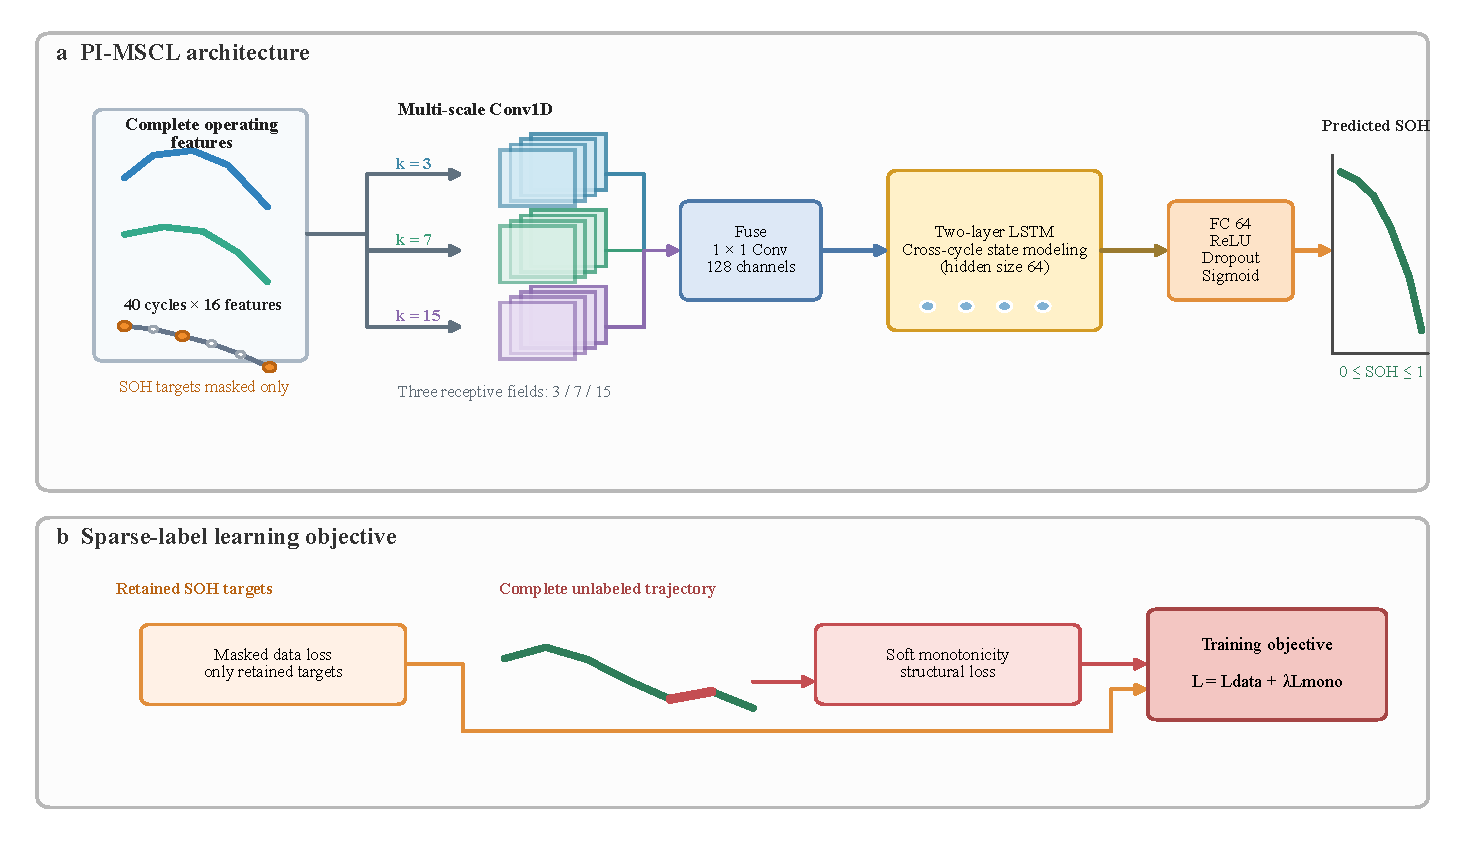
\includegraphics[width=\textwidth]{../../docs/PI-MSCL_architecture_single_column_preview.pdf}
\caption{PI-MSCL under controlled sparse cycle-level supervision. Panel (a) shows the feature-to-SOH mapping. Panel (b) distinguishes masked data fitting from the soft monotonicity term, which is evaluated on valid ordered pairs from the same cell within each mini-batch.}
  \label{fig:pimscl_framework}
\end{figure}

Figure~\ref{fig:pimscl_framework} separates the model from the learning objective. In panel (a), convolutional branches capture short-, medium-, and longer-range patterns before the LSTM maps the fused representation to a cycle-wise SOH estimate. Panel (b) distinguishes masked data fitting from the soft monotonicity term. All feature windows remain in the forward pass. The structural term includes windows whose SOH targets were not retained when they form valid ordered pairs within a mini-batch.

\subsection{Multi-scale representation and temporal state modeling}
\label{subsec:multiscale}

Charging trajectories contain information at more than one temporal scale. Neighbouring cycles capture local charge-response variation; intermediate windows capture shifts in charge duration and voltage statistics; longer windows describe slower changes associated with capacity fade. A single convolutional kernel privileges one receptive field and may not represent these patterns equally well.

To address this issue, PI-MSCL uses a three-branch multi-scale one-dimensional CNN module. Each branch receives the same input sequence but uses a different kernel size:
\begin{equation}
\mathbf{H}^{(s)}_{i,t}=\phi_{s}\left(\mathbf{X}_{i,t};k_s\right),
\quad k_s\in\{3,7,15\},
\label{eq:multiscale_branch}
\end{equation}
where $\phi_s(\cdot)$ denotes a branch containing two repeated Conv1D--batch-normalization--ReLU--max-pooling blocks. Same padding is used in the convolutions, and each pooling layer has kernel size and stride two. The three kernel sizes represent short-, medium-, and long-range receptive fields, respectively, while both convolutional layers in every branch contain 64 channels. For $T=40$, the two pooling operations reduce each aligned branch sequence to 10 temporal positions. The three outputs are concatenated along the channel dimension and fused by a $1\times1$ convolution:
\begin{equation}
\mathbf{H}_{i,t}=\phi_{\mathrm{fuse}}\left(
\left[\mathbf{H}^{(3)}_{i,t};\mathbf{H}^{(7)}_{i,t};\mathbf{H}^{(15)}_{i,t}\right]
\right),
\label{eq:multiscale_fusion}
\end{equation}
where $[\cdot;\cdot;\cdot]$ denotes channel-wise concatenation and $\phi_{\mathrm{fuse}}(\cdot)$ maps the resulting 192 channels to 128 channels using Conv1D, batch normalization, and ReLU activation. This design changes the receptive-field structure without changing the downstream LSTM used by the single- and multi-scale variants.

\noindent\textbf{Temporal state mapping.}
The fused sequence $\mathbf{H}_{i,t}$ is then passed to an LSTM, whose gated state updates retain useful history while filtering transient variation \cite{hochreiter1997long}. PI-MSCL uses two LSTM layers with a hidden dimension of 64:
\begin{equation}
\mathbf{Z}_{i,t}=\mathrm{LSTM}\left(\mathbf{H}_{i,t}\right),
\label{eq:lstm_sequence}
\end{equation}
where $\mathbf{Z}_{i,t}$ denotes the hidden-state sequence. Its last state $\mathbf{z}_{i,t}^{\mathrm{last}}$ represents the input window and is passed to a regression head,
\begin{equation}
\hat{y}_{i,t}=\sigma\left(f_{\mathrm{fc}}\left(\mathbf{z}_{i,t}^{\mathrm{last}}\right)\right),
\label{eq:soh_regression}
\end{equation}
where $f_{\mathrm{fc}}(\cdot)$ comprises a 64-unit fully connected layer, ReLU activation, dropout with probability 0.4, and a scalar output layer; $\sigma(\cdot)$ is the sigmoid function. The sigmoid bounds the predicted SOH to $[0,1]$, matching the normalised capacity target. No separate boundary penalty is used in the main configuration.

The encoder represents every feature window, while the masked data loss and physics-constrained objective determine how those representations enter optimisation. The objective combines a soft monotonicity term with a rate-continuity term, which respectively regulate the direction and local variation of the estimated SOH trajectory. Their construction, hyperparameters, and evaluation are specified in Sections~\ref{subsec:loss_functions} and \ref{subsec:evaluation_metrics}.
\section{Experimental Setup}
\label{sec:experiments}

\subsection{Datasets and SOH definition}
\label{subsec:datasets}

The study uses the public HUST lithium-ion battery degradation dataset \cite{Yuan2022HUSTDataset}. It contains full-lifecycle records from 77 LFP/graphite cells with a nominal capacity of 1.1 Ah and nominal voltage of 3.3 V. The cells were tested at 30~$^{\circ}$C with a common constant-current/constant-voltage charging procedure and multiple discharge profiles. Their lifetimes, fading rates, and local capacity fluctuations differ substantially, which makes cell-level separation necessary for evaluating unseen-cell generalisation. The public dataset also provides a reproducible basis for the analysis \cite{ward2022principles}.

SOH was defined as normalized capacity relative to the initial capacity of each cell:
\begin{equation}
\mathrm{SOH}_{i,t}=\frac{Q_{i,t}}{Q_{i,0}},
\label{eq:soh_definition}
\end{equation}
where $Q_{i,t}$ is the measured capacity of cell $i$ at cycle $t$ and $Q_{i,0}$ is the initial measured capacity. This definition makes the target dimensionless and aligns the prediction range with the sigmoid-bounded output of PI-MSCL.

HUST provides capacity measurements for every recorded cycle. The sparse-label protocol is applied after the cell split and only to training targets. It retains the original feature records and isolates a distributed training-label budget.

Figure~\ref{fig:hust_all_discharge_capacity} shows the normalised discharge-capacity trajectories of all 77 cells. Each line represents one cell. The variation in lifetime, local fluctuation, and late-life decline motivates cell-level separation rather than random window splitting. This descriptive view precedes and is independent of the training-target masking protocol.

\begin{figure}[t]
  \centering
  \includegraphics[width=\textwidth]{../../output/figures/formal_main_v3/fig2_hust_all_discharge_capacity.pdf}
  \caption{Normalised discharge-capacity trajectories of all 77 HUST cells. Each line represents one cell and is normalised by its initial measured capacity.}
  \label{fig:hust_all_discharge_capacity}
\end{figure}

\subsection{Feature construction and preprocessing}
\label{subsec:features_preprocessing}

The analysis uses the 16 charging-cycle features listed in Table~\ref{tab:features}. They describe voltage and current statistics, CC/CV charge throughput and duration, local slopes, and entropy-based signal complexity. The discharge-capacity measurement used to construct SOH is excluded from the input.

\begin{table}[t]
\caption{Charging-cycle features used for SOH estimation.}
\label{tab:features}
\centering
\begin{tabular*}{\textwidth}{@{\extracolsep{\fill}}lll@{}}
\toprule
Group & Feature & Description \\
\midrule
Voltage statistics & voltage mean & Mean voltage during the CC stage \\
Voltage statistics & voltage std & Voltage fluctuation during the CC stage \\
Voltage statistics & voltage kurtosis & Sharpness of the voltage distribution \\
Voltage statistics & voltage skewness & Asymmetry of the voltage distribution \\
CC-stage dynamics & CC Q & Charged capacity during the CC stage \\
CC-stage dynamics & CC charge time & Duration of the CC charging stage \\
Voltage dynamics & voltage slope & Local slope of the charging-voltage signal \\
Voltage complexity & voltage entropy & Entropy-based complexity of the voltage signal \\
Current statistics & current mean & Mean current during the CV stage \\
Current statistics & current std & Current fluctuation during the CV stage \\
Current statistics & current kurtosis & Sharpness of the current distribution \\
Current statistics & current skewness & Asymmetry of the current distribution \\
CV-stage dynamics & CV Q & Charged capacity during the CV stage \\
CV-stage dynamics & CV charge time & Duration of the CV charging stage \\
Current dynamics & current slope & Local slope of the charging-current signal \\
Current complexity & current entropy & Entropy-based complexity of the current signal \\
\bottomrule
\end{tabular*}
\end{table}

The main analysis retains every recorded cycle and applies no synthetic degradation transform. After splitting the cells, a \texttt{StandardScaler} is fitted to the concatenated training-cell features and then applied unchanged to validation and test cells. Fixed-length windows of $T=40$ are generated within each cell, and the SOH at the final position is used as the many-to-one target.

\subsection{Experimental protocol and hyperparameter settings}
\label{subsec:split_protocol}
\label{subsec:training_config}

All experiments use a cell-level 60/20/20 split, yielding 46 training cells, 15 validation cells, and 16 test cells. Every cycle from a given cell remains in the same subset. Test cells are unseen during optimisation, so the reported errors quantify cross-cell generalisation.

After the split, the SOH-label retention ratio $r$ controls the available targets within the training cells. For training cell $i$, a seeded sampler without replacement selects
\begin{equation}
  n_i^{\mathrm{lab}}=\max\left(1,\operatorname{round}(rN_i)\right)
\end{equation}
of its $N_i$ cycle-level targets and assigns $m_{i,t}=1$ to the selected indices. The remaining indicators are zero. The experiment uses $r\in\{1.0,0.7,0.5,0.3\}$, with $r=1.0$ as the full-supervision reference. Feature rows, cycle order, and windows are retained at every ratio. Validation and test cells remain fully labelled for model selection and final evaluation. This design isolates sensitivity to a distributed within-cell SOH-label budget; it is not a temporal-prefix or periodic-calibration protocol.

Cell-split, label-mask, and network-initialisation seeds are recorded separately for every run. The primary matrix fixes the cell split at seed 42 and uses paired training/mask seeds (929/1929), (2262/3262), and (7/1007). Within each repetition, the four factorial variants share the same split and mask. The variants are CNN--LSTM, PI--CNN--LSTM, MS--CNN--LSTM, and PI-MSCL, obtained by switching between single- and multi-scale convolution and by disabling or enabling the soft monotonicity constraint; the rate-continuity weight is fixed at zero in this matrix. Complementary XGBoost, LSTM, GRU, and attention CNN--LSTM baselines use the same data interface and are evaluated at $r=1.0$ and $r=0.3$. The expanded panel is therefore a same-protocol comparison, not an architecture-specific hyperparameter search.

The LSTM and GRU baselines use two recurrent layers with hidden dimension 64 and the common 64-unit regression head. The attention CNN--LSTM uses convolutional channels 256 and 128 with kernel size 7, a two-layer LSTM, and four-head self-attention with dropout 0.1. XGBoost uses 300 trees, depth 6, learning rate 0.05, row/column subsampling of 0.8, and L1/L2 coefficients of 0.1/1.0. Table~\ref{tab:hyperparameters} lists the shared PI-MSCL and training settings used in the formal matrix.

\begin{table}[t]
\caption{Main experimental and model hyperparameters.}
\label{tab:hyperparameters}
\centering
\setlength{\tabcolsep}{5pt}
\renewcommand{\arraystretch}{1.08}
\begin{tabular*}{\textwidth}{@{\extracolsep{\fill}}lll@{}}
\toprule
Category & Hyperparameter & Setting \\
\midrule
Data & Input dimension / window length & 16 / 40 cycles \\
Protocol & Split / label ratios & 60:20:20 / 1.0, 0.7, 0.5, 0.3 \\
Optimization & Optimizer / batch size / epochs & Adam / 1024 / 200 \\
Optimization & Learning-rate schedule & $2\times10^{-3}\rightarrow5\times10^{-3}\rightarrow10^{-4}$ \\
Optimization & Warmup / early-stop patience & 20 / 20 epochs \\
Multi-scale CNN & Kernels / layers per branch & 3, 7, 15 / 2 \\
Multi-scale CNN & Branch / fusion channels & 64 / 128 \\
Temporal head & LSTM layers / hidden units & 2 / 64 \\
Regression head & FC units / dropout & 64 / 0.4 \\
Soft monotonicity & $\lambda_{\mathrm{mono}}$ / $\epsilon$ & 0.3 / 0.005 \\
Soft monotonicity & $c_{\min}$ / $K$ / $\alpha$ & 300 / 40 / 0.2 \\
Rate continuity (M4) & $\lambda_{\mathrm{rate}}$ & 0 (M4: 0.05) \\
\bottomrule
\end{tabular*}
\end{table}

Models are optimised for at most 200 epochs. The learning rate increases linearly during warm-up and then follows cosine decay. Early stopping monitors validation MAE, and the checkpoint with the lowest value is restored for testing. Each formal run archives its configuration, seed roles, cell lists, predictions, targets, cell identifiers, and true cycle indices. Reported values are means and sample standard deviations across the three formal repetitions. The estimates are conditional on the fixed cell split at seed 42.

\subsection{Loss functions}
\label{subsec:loss_functions}

The masked supervised loss in Eq.~\eqref{eq:masked_mse} fits only retained SOH targets. When $m_{i,t}=0$, the target supplies no data-fitting gradient, but its feature window remains in the forward pass. No unretained target is replaced by a model-generated label.

PI-MSCL supplements this masked fit with a soft monotonicity constraint after the early activation region. For each mini-batch, valid ordered pairs are
\begin{equation}
\mathcal{P}=\left\{(a,b): i_a=i_b,\;0<c_b-c_a\leq K,\;c_a\geq c_{\min}\right\},
\label{eq:pair_set}
\end{equation}
where both samples belong to one cell, $K$ limits the cycle gap, and $c_{\min}$ delays activation of the prior. The constraint is
\begin{equation}
\mathcal{L}_{\mathrm{mono}}=
\frac{1}{|\mathcal{P}|}\sum_{(a,b)\in\mathcal{P}}
\exp[-\alpha(c_b-c_a)]
\mathrm{ReLU}\left(\hat{y}_{i_b,c_b}-\hat{y}_{i_a,c_a}-\epsilon\right),
\label{eq:mono_loss}
\end{equation}
where $\epsilon$ permits small local increases and the exponential factor gives closer pairs greater weight. The retention indicator does not enter Eq.~\eqref{eq:mono_loss}; cycles without retained SOH targets can therefore contribute structural, rather than numerical, information.

\noindent\textbf{Rate-continuity constraint.}
The rate-continuity term penalises changes in the discrete first difference of the predicted SOH sequence. For each cell, predictions are ordered by cycle index within a mini-batch. Let $\mathcal{T}$ denote valid consecutive triplets in this ordered sequence whose earliest cycle is at least $c_{\min}$. The term is
\begin{equation}
\mathcal{L}_{\mathrm{rate}}=
\frac{1}{|\mathcal{T}|}\sum_{(a,b,c)\in\mathcal{T}}
\left(\hat{y}_{i,c}-2\hat{y}_{i,b}+\hat{y}_{i,a}\right)^2.
\label{eq:rate_loss}
\end{equation}
It is the squared discrete second difference: minimising it encourages successive SOH changes to vary smoothly and suppresses high-frequency zig-zag behaviour. Together, $\mathcal{L}_{\mathrm{mono}}$ limits implausible upward drift, whereas $\mathcal{L}_{\mathrm{rate}}$ limits abrupt changes in the degradation rate. Both terms use predictions and ordered cycle indices rather than SOH labels, and are evaluated only within a cell. The resulting physics-informed objective is
\begin{equation}
\mathcal{L}=\mathcal{L}_{\mathrm{sup}}+\lambda_{\mathrm{mono}}\mathcal{L}_{\mathrm{mono}}+\lambda_{\mathrm{rate}}\mathcal{L}_{\mathrm{rate}}.
\label{eq:total_loss}
\end{equation}
The M4 configuration uses $\lambda_{\mathrm{rate}}=0.05$.

\subsection{Evaluation metrics and statistical reporting}
\label{subsec:evaluation_metrics}
\label{subsec:metrics}

SOH estimation performance is evaluated using mean absolute error (MAE), root mean squared error (RMSE), and the coefficient of determination ($R^2$):
\begin{align}
\mathrm{MAE} &= \frac{1}{N}\sum_{n=1}^{N}\left|\hat{y}_{n}-y_{n}\right|, \\
\mathrm{RMSE} &= \sqrt{\frac{1}{N}\sum_{n=1}^{N}\left(\hat{y}_{n}-y_{n}\right)^2}, \\
R^2 &= 1-\frac{\sum_{n=1}^{N}\left(y_n-\hat{y}_n\right)^2}{\sum_{n=1}^{N}\left(y_n-\bar{y}\right)^2}.
\end{align}
MAE measures average deviation, RMSE gives greater weight to large errors, and $R^2$ measures explained variance. All three are computed over every window from the fully labelled test cells. Trajectory metrics are computed independently for each test cell after sorting predictions by the saved cycle index. Let $\Delta\hat{y}_{i,t}=\hat{y}_{i,t+1}-\hat{y}_{i,t}$ for adjacent available predictions whose earlier cycle is at least $c_{\min}$. The monotonicity-violation rate, cumulative upward excess, and trajectory roughness are
\begin{align}
V_{\mathrm{mono}} &= 100\,\frac{\sum_{i,t}\mathbb{I}\!\left(\Delta\hat{y}_{i,t}>\epsilon\right)}{N_{\mathrm{pair}}},\\
U_i &= \sum_t \max\left(\Delta\hat{y}_{i,t}-\epsilon,0\right),\\
D_2 &= \frac{1}{N_{\mathrm{trip}}}\sum_{i,t}\left|\hat{y}_{i,t+2}-2\hat{y}_{i,t+1}+\hat{y}_{i,t}\right|.
\end{align}
The analysis reports $V_{\mathrm{mono}}$, $\bar{U}$ (the mean of $U_i$ across test cells), and $D_2$ (the mean absolute second difference over eligible adjacent triplets). The evaluation uses the same $\epsilon=0.005$ and $c_{\min}=300$ as training. Only adjacent pairs are included, giving the violation rate an unambiguous denominator. A representative trajectory is selected in two predeclared stages. First, test MAE is averaged over the four factorial variants for each paired mask/training-seed repetition, and the repetition closest to the median of the three cross-model means is retained. Second, each test cell's MAE is averaged over the four variants within that repetition; the cell closest to the across-cell median is displayed. Seed and cell identifiers resolve any tie. The selected repetition and cell are therefore independent of PI-MSCL performance or trajectory appearance.
\section{Experimental Results and Analysis}
\label{sec:results}

% This result shell intentionally contains no legacy values. Formal values,
% tables, and figures are populated only from non-smoke runs produced after the
% battery-boundary and preprocessing-leakage corrections.
\subsection{Overall cross-cell prediction and error characteristics}
\label{subsec:overall_prediction}

The full-supervision experiment establishes the reference performance on the fixed unseen-cell test set. In Table~\ref{tab:all_models_full_supervision}, PI-MSCL achieved the lowest mean MAE among the eight same-protocol models ($1.556\pm0.044\%$). GRU achieved the lowest RMSE ($2.714\pm0.039\%$) and the highest $R^2$ ($0.8608\pm0.0040$), while attention CNN--LSTM and GRU approached PI-MSCL in MAE. The three metrics therefore resolve different aspects of prediction quality.

\begin{table}[htbp]
\caption{Same-protocol comparison under full supervision. Values are mean $\pm$ sample standard deviation across three paired repetitions on the fixed cell split (seed 42).}
\label{tab:all_models_full_supervision}
\centering
\setlength{\tabcolsep}{3.0pt}
\begin{tabular*}{\textwidth}{@{\extracolsep{\fill}}lccc@{}}
\toprule
Model & MAE (\%) & RMSE (\%) & R-squared \\
\midrule
XGBoost & 1.800 \textpm{} 0.033 & 3.061 \textpm{} 0.053 & 0.8229 \textpm{} 0.0061 \\
LSTM & 1.680 \textpm{} 0.047 & 2.958 \textpm{} 0.074 & 0.8346 \textpm{} 0.0083 \\
GRU & 1.634 \textpm{} 0.032 & 2.714 \textpm{} 0.039 & 0.8608 \textpm{} 0.0040 \\
Attn. CNN--LSTM & 1.633 \textpm{} 0.059 & 2.900 \textpm{} 0.061 & 0.8410 \textpm{} 0.0067 \\
CNN--LSTM & 1.649 \textpm{} 0.050 & 2.948 \textpm{} 0.076 & 0.8357 \textpm{} 0.0085 \\
PI--CNN--LSTM & 1.679 \textpm{} 0.055 & 3.058 \textpm{} 0.109 & 0.8231 \textpm{} 0.0126 \\
MS--CNN--LSTM & 1.582 \textpm{} 0.102 & 3.048 \textpm{} 0.222 & 0.8238 \textpm{} 0.0260 \\
PI--MSCL & 1.556 \textpm{} 0.044 & 2.984 \textpm{} 0.028 & 0.8317 \textpm{} 0.0032 \\
\bottomrule
\end{tabular*}
\end{table}


Figure~\ref{fig:overall_prediction_error} adds sample- and cell-level detail. Panel (a) uses the median-MAE PI-MSCL repetition; its MAE, RMSE, and $R^2$ were 1.541\%, 2.981\%, and 0.8320, respectively. Predictions clustered around the identity line at high SOH, while dispersion and cell-specific bands increased at lower SOH. Panel (b) gives one MAE per unseen cell and model after averaging that cell's error over the three repetitions. PI-MSCL had a median per-cell MAE of 1.300\%, but its most difficult cell reached 4.730\%; the corresponding values for the unconstrained multi-scale model were 1.236\% and 4.704\%. The sample-weighted MAE advantage therefore arose alongside persistent late-life errors in several cells.

\begin{figure}[t]
  \centering
  \includegraphics[width=\textwidth]{../../output/figures/formal_main_v3/fig2_overall_prediction_and_error_group.pdf}
  \caption{Full-supervision prediction agreement and per-cell error distribution on unseen cells. Panel (a) shows the median-MAE PI-MSCL repetition. Panel (b) summarises the MAE of 16 test cells after each cell's error is averaged across the three repetitions; boxes show the median and interquartile range, whiskers extend to 1.5 times the interquartile range, and points show individual cells.}
  \label{fig:overall_prediction_error}
\end{figure}

Together, the table and figure distinguish average accuracy from the distribution of residuals. The multi-scale encoder reduced many moderate deviations, while a small number of difficult cell trajectories continued to dominate RMSE.

\subsection{Label-budget sensitivity and representative-cell behavior}
\label{subsec:new_label_budget}

The factorial comparison resolves how this full-supervision result arose. Within the four related architectures, PI-MSCL had the lowest dense-label mean MAE ($1.556\pm0.044\%$), followed by the unconstrained multi-scale model ($1.582\pm0.102\%$). The single-scale CNN--LSTM instead had the lowest RMSE ($2.948\pm0.076\%$) and the highest $R^2$ ($0.8357\pm0.0085$). Adding the soft constraint increased single-scale MAE and RMSE by 0.030 and 0.110 percentage points, respectively. In the multi-scale model, it reduced MAE and RMSE by 0.026 and 0.064 percentage points; the MAE reduction occurred in one of the three paired repetitions.

The retention curves in Fig.~\ref{fig:label_budget_performance} and Tables~\ref{tab:label_budget_mae}--\ref{tab:label_budget_r2} use the same fully labelled unseen cells while decreasing the available training targets. Performance did not decline monotonically with every reduction in $r$. The single-scale constrained model had the lowest mean MAE at $r=0.7$ and $r=0.5$ (1.588\% and 1.598\%), whereas PI-MSCL led at $r=1.0$. At $r=0.3$, the unconstrained multi-scale model achieved $1.634\pm0.057\%$ MAE, compared with $1.677\pm0.128\%$ for PI-MSCL. Relative to its dense-label reference, PI-MSCL increased by 0.121 percentage points in MAE at 30\% retention. Its $R^2$ changed from 0.8317 to 0.8251, while the standard deviation increased from 0.0032 to 0.0238.

\begin{figure}[t]
  \centering
  \includegraphics[width=\textwidth]{../../output/figures/formal_main_v3/fig3_performance_vs_label_budget_group.pdf}
  \caption{Point-estimation performance across SOH-label retention ratios. Points show means and error bars show sample standard deviations across three paired repetitions on the fixed cell split (seed 42).}
  \label{fig:label_budget_performance}
\end{figure}

\begin{table}[htbp]
\caption{MAE (\%) across SOH-label retention ratios. Values are mean $\pm$ sample standard deviation across three paired repetitions on the fixed cell split (seed 42).}
\label{tab:label_budget_mae}
\centering
\setlength{\tabcolsep}{3.5pt}
\begin{tabular*}{\textwidth}{@{\extracolsep{\fill}}lcccc@{}}
\toprule
Model & r = 1.0 & r = 0.7 & r = 0.5 & r = 0.3 \\
\midrule
CNN--LSTM & 1.649 \textpm{} 0.050 & 1.647 \textpm{} 0.103 & 1.679 \textpm{} 0.138 & 1.659 \textpm{} 0.031 \\
PI--CNN--LSTM & 1.679 \textpm{} 0.055 & 1.588 \textpm{} 0.030 & 1.598 \textpm{} 0.017 & 1.677 \textpm{} 0.021 \\
MS--CNN--LSTM & 1.582 \textpm{} 0.102 & 1.650 \textpm{} 0.076 & 1.614 \textpm{} 0.055 & 1.634 \textpm{} 0.057 \\
PI--MSCL & 1.556 \textpm{} 0.044 & 1.605 \textpm{} 0.029 & 1.659 \textpm{} 0.139 & 1.677 \textpm{} 0.128 \\
\bottomrule
\end{tabular*}
\end{table}

\begin{table}[htbp]
\caption{$R^2$ across SOH-label retention ratios. Values are mean $\pm$ sample standard deviation across three paired repetitions on the fixed cell split (seed 42).}
\label{tab:label_budget_r2}
\centering
\setlength{\tabcolsep}{3.5pt}
\begin{tabular*}{\textwidth}{@{\extracolsep{\fill}}lcccc@{}}
\toprule
Model & r = 1.0 & r = 0.7 & r = 0.5 & r = 0.3 \\
\midrule
CNN--LSTM & 0.8357 \textpm{} 0.0085 & 0.8371 \textpm{} 0.0263 & 0.8350 \textpm{} 0.0200 & 0.8301 \textpm{} 0.0071 \\
PI--CNN--LSTM & 0.8231 \textpm{} 0.0126 & 0.8437 \textpm{} 0.0095 & 0.8426 \textpm{} 0.0163 & 0.8192 \textpm{} 0.0076 \\
MS--CNN--LSTM & 0.8238 \textpm{} 0.0260 & 0.8148 \textpm{} 0.0167 & 0.8310 \textpm{} 0.0134 & 0.8251 \textpm{} 0.0120 \\
PI--MSCL & 0.8317 \textpm{} 0.0032 & 0.8228 \textpm{} 0.0030 & 0.8217 \textpm{} 0.0183 & 0.8251 \textpm{} 0.0238 \\
\bottomrule
\end{tabular*}
\end{table}


The constraint effect varied with label retention and encoder scale. In the single-scale model, it reduced mean MAE by 0.058 and 0.081 percentage points at $r=0.7$ and $r=0.5$, but increased MAE by 0.030 and 0.018 percentage points at $r=1.0$ and $r=0.3$. In the multi-scale model, it reduced MAE by 0.026 and 0.045 percentage points at $r=1.0$ and $r=0.7$, and increased it by 0.044 and 0.043 percentage points at $r=0.5$ and $r=0.3$. These paired contrasts motivate the trajectory analysis below.

Figure~\ref{fig:representative_trajectory} shows the unseen cell selected by the predeclared median-repetition and median-cell rules. The procedure selected training seed 2262, mask seed 3262, and cell 10-6 at $r=0.3$. All variants followed the broad capacity-fade trend, but their late-life residuals differed. The constrained variants suppressed short upward excursions, while the aligned error panel shows that smoother output did not remove local bias. This cell-level view mirrors the accuracy--trajectory-consistency trade-off in the aggregate results.

\begin{figure}[t]
  \centering
  \includegraphics[width=\textwidth]{../../output/figures/formal_main_v3/fig4_trajectory_and_error_group.pdf}
  \caption{Representative unseen-cell SOH trajectory and aligned prediction error at 30\% SOH-label retention. The displayed repetition uses training/mask seeds 2262/3262, and cell 10-6 was selected by the predeclared median-repetition and median-cell rule.}
  \label{fig:representative_trajectory}
\end{figure}

The intervention changes the density of cycle-level targets, while retaining the cells and full feature records at every ratio. Randomly retained targets may occur in early, middle, and late life.

\subsection{Same-protocol endpoint comparison}
\label{subsec:new_extended_baselines}

The endpoint comparison asks whether the factorial-family pattern extends to complementary model classes. XGBoost, LSTM, GRU, and attention CNN--LSTM were evaluated at $r=1.0$ and $r=0.3$ with the same cell split, 16-feature windows, retained-label masks, fully labelled test cells, and paired seeds. Their dense-label results appear in Table~\ref{tab:all_models_full_supervision}; Table~\ref{tab:all_models_endpoint_budget} reports the paired change between the two endpoints.

At 30\% retention, attention CNN--LSTM attained the lowest MAE ($1.567\pm0.087\%$), followed by GRU ($1.599\pm0.042\%$); PI-MSCL reached $1.677\pm0.128\%$. The four complementary baselines had small negative mean endpoint changes, with paired standard deviations of similar magnitude. PI-MSCL instead showed a $+0.121\pm0.125$-percentage-point paired MAE change, indicating greater point-error sensitivity at the smallest label budget.

\begin{table}[htbp]
\caption{Same-protocol endpoint comparison across SOH-label retention ratios. Values are mean $\pm$ sample standard deviation across three paired repetitions on the fixed cell split (seed 42); change is $r=0.3-r=1.0$.}
\label{tab:all_models_endpoint_budget}
\centering
\setlength{\tabcolsep}{3.0pt}
\begin{tabular*}{\textwidth}{@{\extracolsep{\fill}}lccc@{}}
\toprule
Model & \multicolumn{2}{c}{MAE (\%)} & Change (pp) \\
\cmidrule(lr){2-3}
 & r = 1.0 & r = 0.3 & 0.3--1.0 \\
\midrule
XGBoost & 1.800 \textpm{} 0.033 & 1.773 \textpm{} 0.038 & -0.028 \textpm{} 0.067 \\
LSTM & 1.680 \textpm{} 0.047 & 1.630 \textpm{} 0.083 & -0.050 \textpm{} 0.128 \\
GRU & 1.634 \textpm{} 0.032 & 1.599 \textpm{} 0.042 & -0.035 \textpm{} 0.064 \\
Attn. CNN--LSTM & 1.633 \textpm{} 0.059 & 1.567 \textpm{} 0.087 & -0.066 \textpm{} 0.100 \\
CNN--LSTM & 1.649 \textpm{} 0.050 & 1.659 \textpm{} 0.031 & 0.010 \textpm{} 0.039 \\
PI--CNN--LSTM & 1.679 \textpm{} 0.055 & 1.677 \textpm{} 0.021 & -0.002 \textpm{} 0.037 \\
MS--CNN--LSTM & 1.582 \textpm{} 0.102 & 1.634 \textpm{} 0.057 & 0.052 \textpm{} 0.148 \\
PI--MSCL & 1.556 \textpm{} 0.044 & 1.677 \textpm{} 0.128 & 0.121 \textpm{} 0.125 \\
\bottomrule
\end{tabular*}
\end{table}


Across the expanded panel, PI-MSCL provided the lowest dense-label MAE, GRU led dense-label RMSE and $R^2$, and attention CNN--LSTM led sparse-endpoint MAE. The factorial contrasts therefore provide the direct evidence for the soft constraint, whereas the expanded panel positions its point-estimation performance among alternative model classes.

\subsection{Trajectory consistency and physical-effect analysis}
\label{subsec:new_trajectory_results}

Table~\ref{tab:all_models_trajectory_sparse} complements the point-error results with trajectory metrics for all eight models. At $r=0.3$, the single-scale constraint reduced the mean monotonicity-violation rate from $0.796\%$ to $0.443\%$, cumulative upward excess from 5.482 to 1.896 percentage points per cell, and roughness from 0.121 to 0.091 percentage points. The corresponding multi-scale comparison reduced these quantities from $0.886\%$ to $0.537\%$, from 5.510 to 1.901 percentage points, and from 0.148 to 0.125 percentage points. In paired form, PI-MSCL reduced the violation rate by $0.348\pm0.317$ percentage points and cumulative upward excess by $3.609\pm2.652$ percentage points, while MAE changed by $+0.043\pm0.185$ percentage points. All three paired repetitions had the same direction of trajectory-consistency improvement at this endpoint; point-error changes had mixed signs.

\begin{table}[htbp]
\caption{Same-protocol trajectory-consistency metrics at 30\% SOH-label retention. Values are mean $\pm$ sample standard deviation across three paired repetitions on the fixed cell split (seed 42). Upward excess is the mean cumulative excess per test cell; lower values are favourable for all columns.}
\label{tab:all_models_trajectory_sparse}
\centering
\setlength{\tabcolsep}{3.0pt}
\begin{tabular*}{\textwidth}{@{\extracolsep{\fill}}lccc@{}}
\toprule
Model & Mono. viol. (\%) & Upward (pp) & Roughness (pp) \\
\midrule
XGBoost & 6.761 \textpm{} 0.458 & 38.2058 \textpm{} 4.8933 & 0.4158 \textpm{} 0.0180 \\
LSTM & 0.176 \textpm{} 0.161 & 2.5954 \textpm{} 2.5633 & 0.0491 \textpm{} 0.0138 \\
GRU & 0.676 \textpm{} 0.308 & 1.4940 \textpm{} 0.9668 & 0.1270 \textpm{} 0.0173 \\
Attn. CNN--LSTM & 0.631 \textpm{} 0.229 & 3.9860 \textpm{} 2.5279 & 0.1066 \textpm{} 0.0112 \\
CNN--LSTM & 0.796 \textpm{} 0.167 & 5.4815 \textpm{} 2.3409 & 0.1206 \textpm{} 0.0163 \\
PI--CNN--LSTM & 0.443 \textpm{} 0.121 & 1.8956 \textpm{} 0.6364 & 0.0909 \textpm{} 0.0070 \\
MS--CNN--LSTM & 0.886 \textpm{} 0.201 & 5.5098 \textpm{} 2.8293 & 0.1476 \textpm{} 0.0020 \\
PI--MSCL & 0.537 \textpm{} 0.207 & 1.9006 \textpm{} 1.5066 & 0.1248 \textpm{} 0.0094 \\
\bottomrule
\end{tabular*}
\end{table}


Across all models, LSTM attained the lowest mean violation rate ($0.176\%$) and roughness (0.0491 percentage points), while GRU attained the lowest cumulative upward excess (1.4940 percentage points). PI-MSCL ranked between these recurrent baselines and its unconstrained counterpart on the three trajectory measures. XGBoost produced substantially more upward and second-difference variation despite a competitive endpoint response to label removal. The controlled paired contrast therefore isolates the structural effect of the soft constraint from the broader model ranking.

Pointwise accuracy and trajectory consistency diverged at the lowest label budget. At 70\% retention, the constraint improved PI-MSCL MAE and all three trajectory quantities on average. At 30\%, it improved all three trajectory quantities relative to the same unconstrained architecture, while paired MAE changes had mixed signs and a slightly adverse mean. The results show that complete feature trajectories can provide label-independent structural information, but cannot replace numerical targets for local calibration.

\subsection{Factorial ablation and interaction}
\label{subsec:new_factorial_ablation}

The $2\times2$ matrix also quantifies paired marginal effects and the architecture--constraint interaction. For a lower-is-better error metric $q_{ap}(r)$, where $a\in\{0,1\}$ denotes single- or multi-scale convolution and $p\in\{0,1\}$ denotes absence or presence of the soft constraint, the average architecture and constraint effects are
\begin{align}
\Delta_{\mathrm{MS}}(r) &= \tfrac{1}{2}\left[q_{00}(r)-q_{10}(r)+q_{01}(r)-q_{11}(r)\right],\\
\Delta_{\mathrm{PI}}(r) &= \tfrac{1}{2}\left[q_{00}(r)-q_{01}(r)+q_{10}(r)-q_{11}(r)\right].
\end{align}
Positive values indicate an average error reduction. Table~\ref{tab:factorial_effects} and Fig.~\ref{fig:factorial_effects} show that the average multi-scale effect was largest under full supervision (0.095 percentage points) and approached zero or changed sign at smaller budgets. The mean constraint effect was small under full supervision ($-0.002$ percentage points), positive at $r=0.7$ and $r=0.5$ (0.052 and 0.018 percentage points), and negative at $r=0.3$ ($-0.031$ percentage points). The architecture--constraint interaction was negative at $r=0.5$ and variable across repetitions. The two modules therefore did not act as independently additive improvements in the tested matrix.

\begin{table}[htbp]
\caption{Paired factorial effects on MAE. Positive main effects indicate lower MAE after adding the corresponding component. Values are mean $\pm$ sample standard deviation across three paired repetitions on the fixed cell split (seed 42).}
\label{tab:factorial_effects}
\centering
\setlength{\tabcolsep}{3.5pt}
\begin{tabular*}{\textwidth}{@{\extracolsep{\fill}}lccc@{}}
\toprule
r & MS effect (pp) & PI effect (pp) & Interaction (pp) \\
\midrule
1.0 & 0.095 \textpm{} 0.047 & -0.002 \textpm{} 0.116 & 0.057 \textpm{} 0.022 \\
0.7 & -0.010 \textpm{} 0.097 & 0.052 \textpm{} 0.017 & -0.013 \textpm{} 0.155 \\
0.5 & 0.003 \textpm{} 0.031 & 0.018 \textpm{} 0.026 & -0.125 \textpm{} 0.334 \\
0.3 & 0.012 \textpm{} 0.025 & -0.031 \textpm{} 0.077 & -0.024 \textpm{} 0.220 \\
\bottomrule
\end{tabular*}
\end{table}


\begin{figure}[t]
  \centering
  \includegraphics[width=\textwidth]{../../output/figures/formal_main_v3/fig5_ablation_effects_group.pdf}
  \caption{Paired effects of multi-scale representation and the soft monotonicity constraint on MAE. Positive values indicate a reduction in MAE. Panel (a) shows the architecture effect $\Delta_{\mathrm{MS}}$ (single-scale minus multi-scale), computed separately without and with the soft constraint. Panel (b) shows the constraint effect $\Delta_{\mathrm{PI}}$ (unconstrained minus constrained), computed separately for the single- and multi-scale architectures. Points show means and error bars show sample standard deviations across three paired repetitions on the fixed cell split (seed 42).}
  \label{fig:factorial_effects}
\end{figure}

The multi-scale representation altered the error distribution rather than improving every metric. Relative to the single-scale data-driven model, it reduced mean MAE at three of four budgets, while its mean RMSE was higher and $R^2$ lower at all four. This agrees with the pooled and cell-level evidence in Fig.~\ref{fig:overall_prediction_error}: wider receptive fields reduced many moderate deviations without removing difficult cell-specific tails.

The results concern a random, distributed cycle-level label budget on the HUST LFP dataset with one fixed cell split. Their transfer to prefix-label, scheduled-calibration, and naturally missing field protocols requires direct validation.

% Two sections archived here on 2026-08-06 during the sparse-label protocol
% rewrite: (1) the pre-rewrite full-supervision benchmark / 2D ablation /
% trajectory case study, and (2) the trajectory-based abnormal-degradation
% risk-indication section (in-house dataset). Full text preserved at
% docs/archived_manuscript_sections_20260806.tex; not \input here because
% neither is in scope for the controlled sparse-label HUST study below.

\section{Conclusion}
\label{sec:conclusion}

This study examined cross-cell lithium-ion battery SOH estimation under a controlled sparse cycle-level supervision protocol. PI-MSCL combines three temporal convolutional scales, recurrent state modelling, masked data fitting, and a soft monotonicity constraint. The design separates cells before model development, retains targets randomly within each training cell, and evaluates fully labelled unseen cells.

PI-MSCL achieved the lowest mean MAE among the eight same-protocol models under full supervision, whereas GRU achieved the lowest RMSE and highest $R^2$. The factorial results showed that the soft constraint improved PI-MSCL MAE and all three trajectory-consistency measures at 70\% retention. At 30\% retention, it continued to reduce monotonicity violations, cumulative upward excess, and roughness relative to the same unconstrained architecture, while paired MAE changes were mixed. Multi-scale representation and the soft constraint were consequently not independently additive across all label budgets.

The adverse mean MAE change for PI-MSCL at 30\% retention (Section~\ref{subsec:new_extended_baselines}) is consistent with two, non-exclusive, mechanisms. First, at the sparsest budget the retained-target sample per cell is small enough that the constraint gradient, which is computed on every ordered pair regardless of label availability, can outweigh the data-fitting gradient during early training and pull point predictions away from the few available numerical anchors even as it keeps the trajectory monotonic. Second, the multi-scale encoder has more parameters than the single-scale baseline, so it may be more sensitive to the reduced effective batch diversity at $r=0.3$; the larger repetition-to-repetition standard deviation for PI-MSCL at this ratio (0.128 percentage points, versus 0.044 at $r=1.0$) is consistent with higher training variance rather than a systematic bias. Distinguishing between these mechanisms would require gradient-magnitude diagnostics or a $\lambda_{\mathrm{mono}}$ sweep at fixed $r$, which we leave to future work.

These findings identify a conditional accuracy--trajectory-consistency trade-off under a distributed within-cell label budget. The soft constraint supplies structural information from ordered feature windows, but local accuracy still depends on numerical SOH anchors. In practice, this suggests a retention-dependent design choice rather than a fixed recommendation: at moderate-to-full retention ($r\geq0.7$), a purely data-driven multi-scale architecture already gives competitive point accuracy at lower implementation complexity, whereas at the sparsest budgets tested, the soft constraint remains preferable whenever trajectory smoothness is the operational priority (e.g., for BMS-facing degradation trends), even though it is not guaranteed to lower point-wise MAE. Future studies should repeat the paired matrix across independent cell partitions, external chemistries, and predeclared prefix-label or periodic-calibration protocols.

\backmatter

\section*{Declarations}

\noindent\textbf{Authors' contributions.}
Chang Liu contributed to conceptualization, investigation, methodology, software, validation, visualization, and writing---original draft. Congyan Chen contributed to formal analysis, funding acquisition, project administration, supervision, validation, and writing---review and editing.

\noindent\textbf{Funding.}
This work was supported by the Guangdong Basic and Applied Basic Research Foundation (Grant No.~2024A1515011962).

\noindent\textbf{Competing interests.}
The authors declare no competing interests.

\noindent\textbf{Data availability.}
The HUST battery dataset is publicly available through Mendeley Data at \url{https://doi.org/10.17632/nsc7hnsg4s.2} \cite{Yuan2022HUSTDataset}. No private or in-house battery dataset is used in the main study.

\noindent\textbf{Code availability.}
The code-availability statement and repository identifier will be confirmed before submission.

\bibliography{references}

\end{document}








